\documentclass[12pt,a4paper]{article}
\usepackage[T2A]{fontenc}
\usepackage[utf8]{inputenc}
\usepackage[russian]{babel}
\usepackage{amsmath,amssymb,geometry,hyperref}
\usepackage[table]{xcolor}
\usepackage{graphicx,fvextra}
\graphicspath{{report-assets/}{./}}
\geometry{margin=18mm}
\setlength{\parindent}{0pt}
\setlength{\parskip}{5pt}
\begin{document}
\begin{center}\large Методы оптимизации\\Отчёт по теме 1. Вариант 4\end{center}
Борисюк Е. Г.
\par\textbf{Условие}\par
\[
z=3x_1+x_2+4x_3+2x_4\to\min,\qquad
\begin{cases}
2x_1+x_2+x_3\le8,\\
x_1+x_3+x_4=5,\\
x_2+x_4\ge4,\\
x_i\ge0.
\end{cases}
\]
\par\textbf{Канонический вид}\par

Добавляю запас $s_1$ в первое ограничение, вычитаю избыток $s_3$ из третьего. Второе уже является равенством.
\[
2x_1+x_2+x_3+s_1=8,\quad
x_1+x_3+x_4=5,\quad
x_2+x_4-s_3=4.
\]
\par\textbf{Вспомогательная задача}\par

Для начального базиса добавляю $a_2,a_3$.
\[
w=a_2+a_3\to\min,\qquad
\begin{cases}
2x_1+x_2+x_3+s_1=8,\\
x_1+x_3+x_4+a_2=5,\\
x_2+x_4-s_3+a_3=4.
\end{cases}
\]
Все переменные неотрицательны. Начальный базис:
$s_1=8,\ a_2=5,\ a_3=4$, остальные переменные равны нулю.

Оценки: $r_j=c_j-\sum_i c_{B_i}t_{ij}$.
Выбираю первый столбец с $r_j<0$, строку по минимуму $b_i/t_{ik}$ при $t_{ik}>0$.
Выделение: голубой — разрешающий столбец, жёлтый — разрешающая строка, оранжевый — разрешающий элемент.
\par\textbf{Таблица I$_{0}$}\begin{center}\small\setlength{\tabcolsep}{4pt}\begin{tabular}{c|rrrrrrrr|r}\hline
Базис & \cellcolor{cyan!18}$x_{1}$ & $x_{2}$ & $x_{3}$ & $x_{4}$ & $s_{1}$ & $s_{3}$ & $a_{2}$ & $a_{3}$ & $b$\\\hline
\rowcolor{yellow!25}$s_{1}$ & \cellcolor{orange!45}$2$ & $1$ & $1$ & $0$ & $1$ & $0$ & $0$ & $0$ & $8$\\
$a_{2}$ & \cellcolor{cyan!18}$1$ & $0$ & $1$ & $1$ & $0$ & $0$ & $1$ & $0$ & $5$\\
$a_{3}$ & \cellcolor{cyan!18}$0$ & $1$ & $0$ & $1$ & $0$ & $-1$ & $0$ & $1$ & $4$\\
\hline $r_j$ & \cellcolor{cyan!18}$-1$ & $-1$ & $-1$ & $-2$ & $0$ & $1$ & $0$ & $0$ & $9$\\\hline\end{tabular}\end{center}
\[\theta_{1}=8/(2)=4,\quad \theta_{2}=5/(1)=5.\]
$x_{1}$ входит, $s_{1}$ выходит. Разрешающий элемент $2$.
{\small\[R_{1}'=R_{1}/(2),\quad R_{2}'=R_{2}-(1)R_{1}'.\]}
\newpage
\par\textbf{Таблица I$_{1}$}\begin{center}\small\setlength{\tabcolsep}{4pt}\begin{tabular}{c|rrrrrrrr|r}\hline
Базис & $x_{1}$ & \cellcolor{cyan!18}$x_{2}$ & $x_{3}$ & $x_{4}$ & $s_{1}$ & $s_{3}$ & $a_{2}$ & $a_{3}$ & $b$\\\hline
$x_{1}$ & $1$ & \cellcolor{cyan!18}$\frac{1}{2}$ & $\frac{1}{2}$ & $0$ & $\frac{1}{2}$ & $0$ & $0$ & $0$ & $4$\\
$a_{2}$ & $0$ & \cellcolor{cyan!18}$\frac{-1}{2}$ & $\frac{1}{2}$ & $1$ & $\frac{-1}{2}$ & $0$ & $1$ & $0$ & $1$\\
\rowcolor{yellow!25}$a_{3}$ & $0$ & \cellcolor{orange!45}$1$ & $0$ & $1$ & $0$ & $-1$ & $0$ & $1$ & $4$\\
\hline $r_j$ & $0$ & \cellcolor{cyan!18}$\frac{-1}{2}$ & $\frac{-1}{2}$ & $-2$ & $\frac{1}{2}$ & $1$ & $0$ & $0$ & $5$\\\hline\end{tabular}\end{center}
\[\theta_{1}=4/(\frac{1}{2})=8,\quad \theta_{3}=4/(1)=4.\]
$x_{2}$ входит, $a_{3}$ выходит. Разрешающий элемент $1$.
{\small\[R_{3}'=R_{3}/(1),\quad R_{1}'=R_{1}-(\frac{1}{2})R_{3}',\quad R_{2}'=R_{2}-(\frac{-1}{2})R_{3}'.\]}
\par\textbf{Таблица I$_{2}$}\begin{center}\small\setlength{\tabcolsep}{4pt}\begin{tabular}{c|rrrrrrrr|r}\hline
Базис & $x_{1}$ & $x_{2}$ & \cellcolor{cyan!18}$x_{3}$ & $x_{4}$ & $s_{1}$ & $s_{3}$ & $a_{2}$ & $a_{3}$ & $b$\\\hline
\rowcolor{yellow!25}$x_{1}$ & $1$ & $0$ & \cellcolor{orange!45}$\frac{1}{2}$ & $\frac{-1}{2}$ & $\frac{1}{2}$ & $\frac{1}{2}$ & $0$ & $\frac{-1}{2}$ & $2$\\
$a_{2}$ & $0$ & $0$ & \cellcolor{cyan!18}$\frac{1}{2}$ & $\frac{3}{2}$ & $\frac{-1}{2}$ & $\frac{-1}{2}$ & $1$ & $\frac{1}{2}$ & $3$\\
$x_{2}$ & $0$ & $1$ & \cellcolor{cyan!18}$0$ & $1$ & $0$ & $-1$ & $0$ & $1$ & $4$\\
\hline $r_j$ & $0$ & $0$ & \cellcolor{cyan!18}$\frac{-1}{2}$ & $\frac{-3}{2}$ & $\frac{1}{2}$ & $\frac{1}{2}$ & $0$ & $\frac{1}{2}$ & $3$\\\hline\end{tabular}\end{center}
\[\theta_{1}=2/(\frac{1}{2})=4,\quad \theta_{2}=3/(\frac{1}{2})=6.\]
$x_{3}$ входит, $x_{1}$ выходит. Разрешающий элемент $\frac{1}{2}$.
{\small\[R_{1}'=R_{1}/(\frac{1}{2}),\quad R_{2}'=R_{2}-(\frac{1}{2})R_{1}'.\]}
\newpage
\par\textbf{Таблица I$_{3}$}\begin{center}\small\setlength{\tabcolsep}{4pt}\begin{tabular}{c|rrrrrrrr|r}\hline
Базис & $x_{1}$ & $x_{2}$ & $x_{3}$ & \cellcolor{cyan!18}$x_{4}$ & $s_{1}$ & $s_{3}$ & $a_{2}$ & $a_{3}$ & $b$\\\hline
$x_{3}$ & $2$ & $0$ & $1$ & \cellcolor{cyan!18}$-1$ & $1$ & $1$ & $0$ & $-1$ & $4$\\
\rowcolor{yellow!25}$a_{2}$ & $-1$ & $0$ & $0$ & \cellcolor{orange!45}$2$ & $-1$ & $-1$ & $1$ & $1$ & $1$\\
$x_{2}$ & $0$ & $1$ & $0$ & \cellcolor{cyan!18}$1$ & $0$ & $-1$ & $0$ & $1$ & $4$\\
\hline $r_j$ & $1$ & $0$ & $0$ & \cellcolor{cyan!18}$-2$ & $1$ & $1$ & $0$ & $0$ & $1$\\\hline\end{tabular}\end{center}
\[\theta_{2}=1/(2)=\frac{1}{2},\quad \theta_{3}=4/(1)=4.\]
$x_{4}$ входит, $a_{2}$ выходит. Разрешающий элемент $2$.
{\small\[R_{2}'=R_{2}/(2),\quad R_{1}'=R_{1}-(-1)R_{2}',\quad R_{3}'=R_{3}-(1)R_{2}'.\]}
\par\textbf{Таблица I$_{4}$}\begin{center}\small\setlength{\tabcolsep}{4pt}\begin{tabular}{c|rrrrrrrr|r}\hline
Базис & $x_{1}$ & $x_{2}$ & $x_{3}$ & $x_{4}$ & $s_{1}$ & $s_{3}$ & $a_{2}$ & $a_{3}$ & $b$\\\hline
$x_{3}$ & $\frac{3}{2}$ & $0$ & $1$ & $0$ & $\frac{1}{2}$ & $\frac{1}{2}$ & $\frac{1}{2}$ & $\frac{-1}{2}$ & $\frac{9}{2}$\\
$x_{4}$ & $\frac{-1}{2}$ & $0$ & $0$ & $1$ & $\frac{-1}{2}$ & $\frac{-1}{2}$ & $\frac{1}{2}$ & $\frac{1}{2}$ & $\frac{1}{2}$\\
$x_{2}$ & $\frac{1}{2}$ & $1$ & $0$ & $0$ & $\frac{1}{2}$ & $\frac{-1}{2}$ & $\frac{-1}{2}$ & $\frac{1}{2}$ & $\frac{7}{2}$\\
\hline $r_j$ & $0$ & $0$ & $0$ & $0$ & $0$ & $0$ & $1$ & $1$ & $0$\\\hline\end{tabular}\end{center}
$w^*=0$, искусственные переменные равны нулю и выведены из базиса.
\newpage
\par\textbf{Основная задача}\par


$w^*=0$, поэтому исходная задача допустима. Удаляю столбцы $a_2,a_3$.
\par Получен план $(0,7/2,9/2,1/2)$.
\par Возвращаю $c=(3,1,4,2,0,0)$; $c_B=(4,2,1)$.
\par Пересчитываю оценки; $z=45/2$.
\par\textbf{Таблица II$_{0}$}\begin{center}\small\setlength{\tabcolsep}{4pt}\begin{tabular}{c|rrrrrr|r}\hline
Базис & \cellcolor{cyan!18}$x_{1}$ & $x_{2}$ & $x_{3}$ & $x_{4}$ & $s_{1}$ & $s_{3}$ & $b$\\\hline
\rowcolor{yellow!25}$x_{3}$ & \cellcolor{orange!45}$\frac{3}{2}$ & $0$ & $1$ & $0$ & $\frac{1}{2}$ & $\frac{1}{2}$ & $\frac{9}{2}$\\
$x_{4}$ & \cellcolor{cyan!18}$\frac{-1}{2}$ & $0$ & $0$ & $1$ & $\frac{-1}{2}$ & $\frac{-1}{2}$ & $\frac{1}{2}$\\
$x_{2}$ & \cellcolor{cyan!18}$\frac{1}{2}$ & $1$ & $0$ & $0$ & $\frac{1}{2}$ & $\frac{-1}{2}$ & $\frac{7}{2}$\\
\hline $r_j$ & \cellcolor{cyan!18}$\frac{-5}{2}$ & $0$ & $0$ & $0$ & $\frac{-3}{2}$ & $\frac{-1}{2}$ & $\frac{45}{2}$\\\hline\end{tabular}\end{center}
\[\theta_{1}=\frac{9}{2}/(\frac{3}{2})=3,\quad \theta_{3}=\frac{7}{2}/(\frac{1}{2})=7.\]
$x_{1}$ входит, $x_{3}$ выходит. Разрешающий элемент $\frac{3}{2}$.
{\small\[R_{1}'=R_{1}/(\frac{3}{2}),\quad R_{2}'=R_{2}-(\frac{-1}{2})R_{1}',\quad R_{3}'=R_{3}-(\frac{1}{2})R_{1}'.\]}
\par\textbf{Таблица II$_{1}$}\begin{center}\small\setlength{\tabcolsep}{4pt}\begin{tabular}{c|rrrrrr|r}\hline
Базис & $x_{1}$ & $x_{2}$ & $x_{3}$ & $x_{4}$ & \cellcolor{cyan!18}$s_{1}$ & $s_{3}$ & $b$\\\hline
$x_{1}$ & $1$ & $0$ & $\frac{2}{3}$ & $0$ & \cellcolor{cyan!18}$\frac{1}{3}$ & $\frac{1}{3}$ & $3$\\
$x_{4}$ & $0$ & $0$ & $\frac{1}{3}$ & $1$ & \cellcolor{cyan!18}$\frac{-1}{3}$ & $\frac{-1}{3}$ & $2$\\
\rowcolor{yellow!25}$x_{2}$ & $0$ & $1$ & $\frac{-1}{3}$ & $0$ & \cellcolor{orange!45}$\frac{1}{3}$ & $\frac{-2}{3}$ & $2$\\
\hline $r_j$ & $0$ & $0$ & $\frac{5}{3}$ & $0$ & \cellcolor{cyan!18}$\frac{-2}{3}$ & $\frac{1}{3}$ & $15$\\\hline\end{tabular}\end{center}
\[\theta_{1}=3/(\frac{1}{3})=9,\quad \theta_{3}=2/(\frac{1}{3})=6.\]
$s_{1}$ входит, $x_{2}$ выходит. Разрешающий элемент $\frac{1}{3}$.
{\small\[R_{3}'=R_{3}/(\frac{1}{3}),\quad R_{1}'=R_{1}-(\frac{1}{3})R_{3}',\quad R_{2}'=R_{2}-(\frac{-1}{3})R_{3}'.\]}
\newpage
\par\textbf{Таблица II$_{2}$}\begin{center}\small\setlength{\tabcolsep}{4pt}\begin{tabular}{c|rrrrrr|r}\hline
Базис & $x_{1}$ & $x_{2}$ & $x_{3}$ & $x_{4}$ & $s_{1}$ & \cellcolor{cyan!18}$s_{3}$ & $b$\\\hline
\rowcolor{yellow!25}$x_{1}$ & $1$ & $-1$ & $1$ & $0$ & $0$ & \cellcolor{orange!45}$1$ & $1$\\
$x_{4}$ & $0$ & $1$ & $0$ & $1$ & $0$ & \cellcolor{cyan!18}$-1$ & $4$\\
$s_{1}$ & $0$ & $3$ & $-1$ & $0$ & $1$ & \cellcolor{cyan!18}$-2$ & $6$\\
\hline $r_j$ & $0$ & $2$ & $1$ & $0$ & $0$ & \cellcolor{cyan!18}$-1$ & $11$\\\hline\end{tabular}\end{center}
\[\theta_{1}=1/(1)=1.\]
$s_{3}$ входит, $x_{1}$ выходит. Разрешающий элемент $1$.
{\small\[R_{1}'=R_{1}/(1),\quad R_{2}'=R_{2}-(-1)R_{1}',\quad R_{3}'=R_{3}-(-2)R_{1}'.\]}
\par\textbf{Таблица II$_{3}$}\begin{center}\small\setlength{\tabcolsep}{4pt}\begin{tabular}{c|rrrrrr|r}\hline
Базис & $x_{1}$ & $x_{2}$ & $x_{3}$ & $x_{4}$ & $s_{1}$ & $s_{3}$ & $b$\\\hline
$s_{3}$ & $1$ & $-1$ & $1$ & $0$ & $0$ & $1$ & $1$\\
$x_{4}$ & $1$ & $0$ & $1$ & $1$ & $0$ & $0$ & $5$\\
$s_{1}$ & $2$ & $1$ & $1$ & $0$ & $1$ & $0$ & $8$\\
\hline $r_j$ & $1$ & $1$ & $2$ & $0$ & $0$ & $0$ & $10$\\\hline\end{tabular}\end{center}

Все оценки неотрицательны. Базис: $s_3=1,\ x_4=5,\ s_1=8$.
Небазисные $x_1=x_2=x_3=0$.
\[
\boxed{x^*=(0,0,0,5),\qquad z_{\min}=10.}
\]
Проверка: $0\le8$, $0+0+5=5$, $0+5\ge4$.
Excel Solver даёт тот же ответ.


\newpage
\par\textbf{Двойственная задача: построение}\par

Исходная задача имеет три ограничения и четыре неотрицательные переменные.
Двойственная имеет три переменные $y_1,y_2,y_3$ и четыре ограничения.
Минимизация заменяется максимизацией. Правые части исходных ограничений
становятся коэффициентами цели:
\[
D=8y_1+5y_2+4y_3\to\max.
\]
Для исходной задачи на минимум ограничению $\le$ соответствует $y_i\le0$,
равенству --- переменная любого знака, ограничению $\ge$ --- $y_i\ge0$:
\[
y_1\le0,\qquad y_2\in\mathbb R,\qquad y_3\ge0.
\]
Каждый столбец исходной матрицы даёт одно двойственное ограничение.
Справа ставлю коэффициент соответствующей переменной в исходной цели:
\[
\begin{array}{c|c|c}
\text{Переменная}&\text{Столбец исходной матрицы}&\text{Ограничение}\\\hline
x_1&(2,1,0)^T&2y_1+y_2\le3\\
x_2&(1,0,1)^T&y_1+y_3\le1\\
x_3&(1,1,0)^T&y_1+y_2\le4\\
x_4&(0,1,1)^T&y_2+y_3\le2
\end{array}
\]
Все четыре знака $\le$, поскольку исходные переменные неотрицательны,
а исходная задача --- на минимум. Итак:
\[
\boxed{D=8y_1+5y_2+4y_3\to\max,}
\qquad
\begin{cases}
2y_1+y_2\le3,\\
y_1+y_3\le1,\\
y_1+y_2\le4,\\
y_2+y_3\le2,\\
y_1\le0,\quad y_2\in\mathbb R,\quad y_3\ge0.
\end{cases}
\]
Знаки двойственных переменных позволяют умножить исходные ограничения
так, чтобы получить нижнюю оценку цели. Складывая их, получаю:
\[
\begin{aligned}
D&\le(2y_1+y_2)x_1+(y_1+y_3)x_2\\
&\quad +(y_1+y_2)x_3+(y_2+y_3)x_4\le z.
\end{aligned}
\]
Следовательно, для любой пары допустимых точек $D(y)\le z(x)$.
Это свойство слабой двойственности.
\newpage
\par\textbf{Двойственная задача: решение и проверка}\par

Из четвёртого ограничения $y_2+y_3\le2$. Переписываю цель:
\[
D=8y_1+5(y_2+y_3)-y_3.
\]
Так как $8y_1\le0$, $5(y_2+y_3)\le10$ и $-y_3\le0$, то
\[
D\le10.
\]
Чтобы достичь этой границы, беру $y_1=0$, $y_3=0$ и $y_2+y_3=2$.
Получаю кандидат $y=(0,2,0)$. Проверяю все ограничения:
\[
\begin{aligned}
2\cdot0+2&=2\le3,\\
0+0&=0\le1,\\
0+2&=2\le4,\\
2+0&=2\le2.
\end{aligned}
\]
Условия на знаки также выполнены. Значение цели:
\[
D(0,2,0)=8\cdot0+5\cdot2+4\cdot0=10.
\]
Граница 10 достигнута в допустимой точке, поэтому
\[
\boxed{y^*=(0,2,0),\qquad D_{\max}=10=z_{\min}.}
\]
Исходная и двойственная точки допустимы, их цели совпадают.
По слабой двойственности это доказывает оптимальность обеих точек.

\par\textbf{Условия дополняющей нежёсткости}\par

При $x^*=(0,0,0,5)$ первое ограничение имеет запас 8, третье --- избыток 1.
Поэтому соответствующие двойственные переменные должны быть нулевыми:
\[
y_1(8-2x_1-x_2-x_3)=0\cdot8=0,
\]
\[
y_3(x_2+x_4-4)=0\cdot1=0.
\]
Так как $x_4=5>0$, четвёртое двойственное ограничение должно быть равенством:
$y_2+y_3=2$. С учётом $y_3=0$ получаю $y_2=2$.
Полная проверка по исходным переменным:
\[
\begin{aligned}
x_1(3-2y_1-y_2)&=0\cdot1=0,\\
x_2(1-y_1-y_3)&=0\cdot1=0,\\
x_3(4-y_1-y_2)&=0\cdot2=0,\\
x_4(2-y_2-y_3)&=5\cdot0=0.
\end{aligned}
\]
Все условия выполнены. Двойственная задача решена аналитически.
\newpage
\par\textbf{Решение в Excel}\par

Переменные находятся в ячейках B5:E5. Цель в B7:
\begin{Verbatim}[fontsize=\small]
=SUMPRODUCT(B5:E5,B6:E6)
\end{Verbatim}
Левые части ограничений в F11:F13 вычисляются по аналогичной формуле.
SUMPRODUCT только вычисляет выражения; оптимальные переменные находит
надстройка <<Поиск решения>> (Solver).

Настройки Solver: целевая ячейка B7, минимум; изменяемые ячейки B5:E5;
ограничения F11 $\le$ H11, F12 $=$ H12, F13 $\ge$ H13, B5:E5 $\ge0$;
метод <<Симплекс LP>>.

Solver дал $x^*=(0,0,0,5)$, $z=10$. Левые части ограничений равны $0,5,5$.
Ответ совпал с ручным решением.
\begin{center}
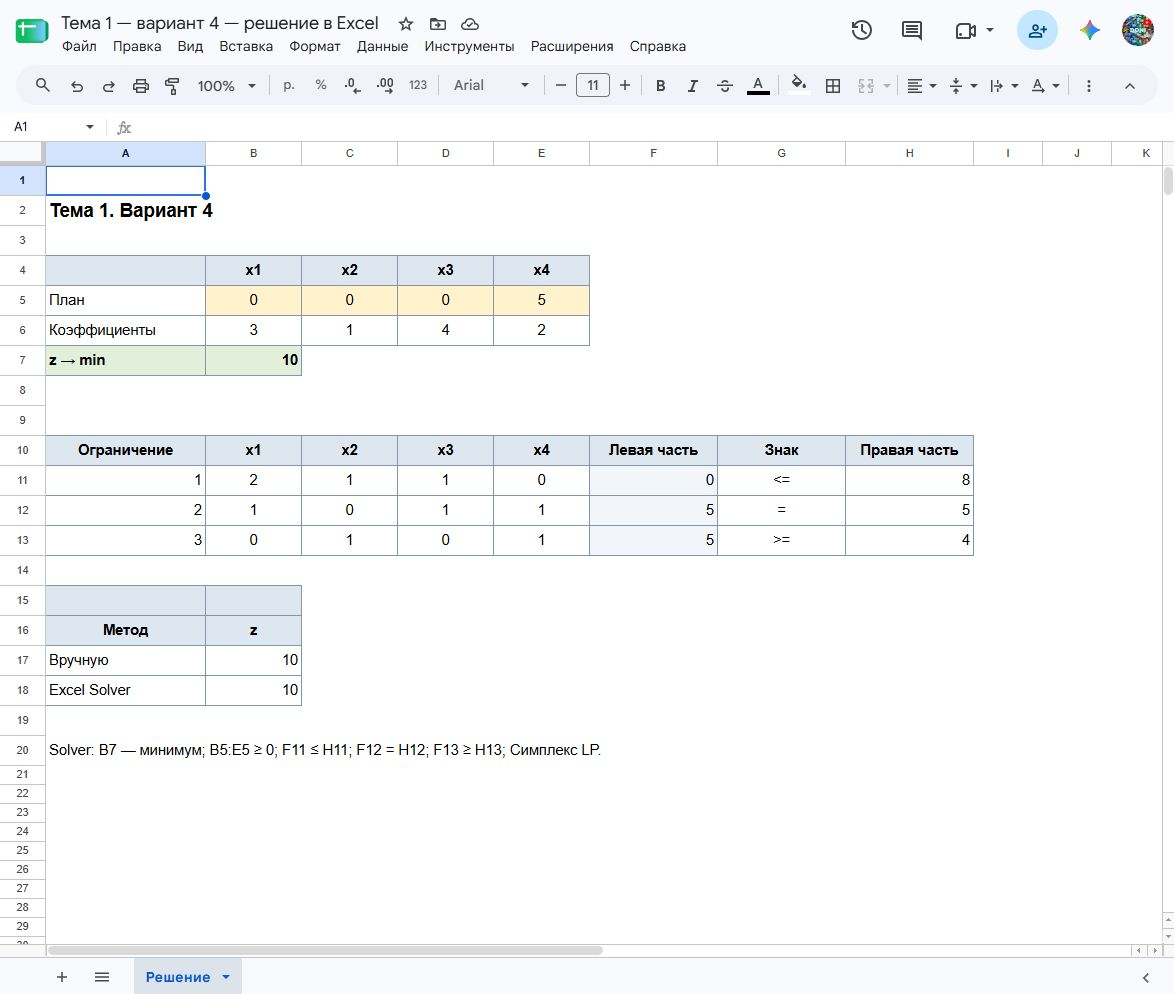
\includegraphics[width=\linewidth]{excel.png}
\end{center}
\small На скриншоте --- копия решённого Excel-файла в Google Таблицах.
\normalsize
\href{https://docs.google.com/spreadsheets/d/1WLAlplmo3eJqNW-X2OTCDIMmLBbabtrBDUC9Oxldsxk/edit}{Открыть таблицу по ссылке}.
\newpage
\par\textbf{Решение на Python в Google Colab}\par

Реализован собственный двухэтапный симплекс-метод.
Данные варианта задаются отдельно от алгоритма. Для точной арифметики
используется стандартный тип Fraction; готовые библиотеки симплекс-метода
не применяются.

Этапы выделены в функции: \texttt{canonicalize} --- канонический вид;
\texttt{auxiliary\_problem} --- вспомогательная задача;
\texttt{reduced\_costs} --- оценки и цель;
\texttt{pivot} --- пересчёт таблицы;
\texttt{simplex} --- выбор переходов;
\texttt{main\_problem} --- удаление искусственных переменных;
\texttt{solve\_lp} --- обе фазы и считывание ответа.

Входящий столбец выбирается по первому отрицательному индексу оценки.
Выходящая строка --- по минимальному отношению при положительном
коэффициенте. При равенстве отношений используется индекс базисной переменной.
Все промежуточные таблицы сохраняются для сравнения с ручным решением.

\par\textbf{Результат выполнения программы}\par

На первой фазе вспомогательная цель менялась как $9,5,3,1,0$.
На второй фазе исходная цель менялась как $45/2,15,11,10$.
Получено семь переходов и девять таблиц, совпадающих с ручным решением.
\begin{center}
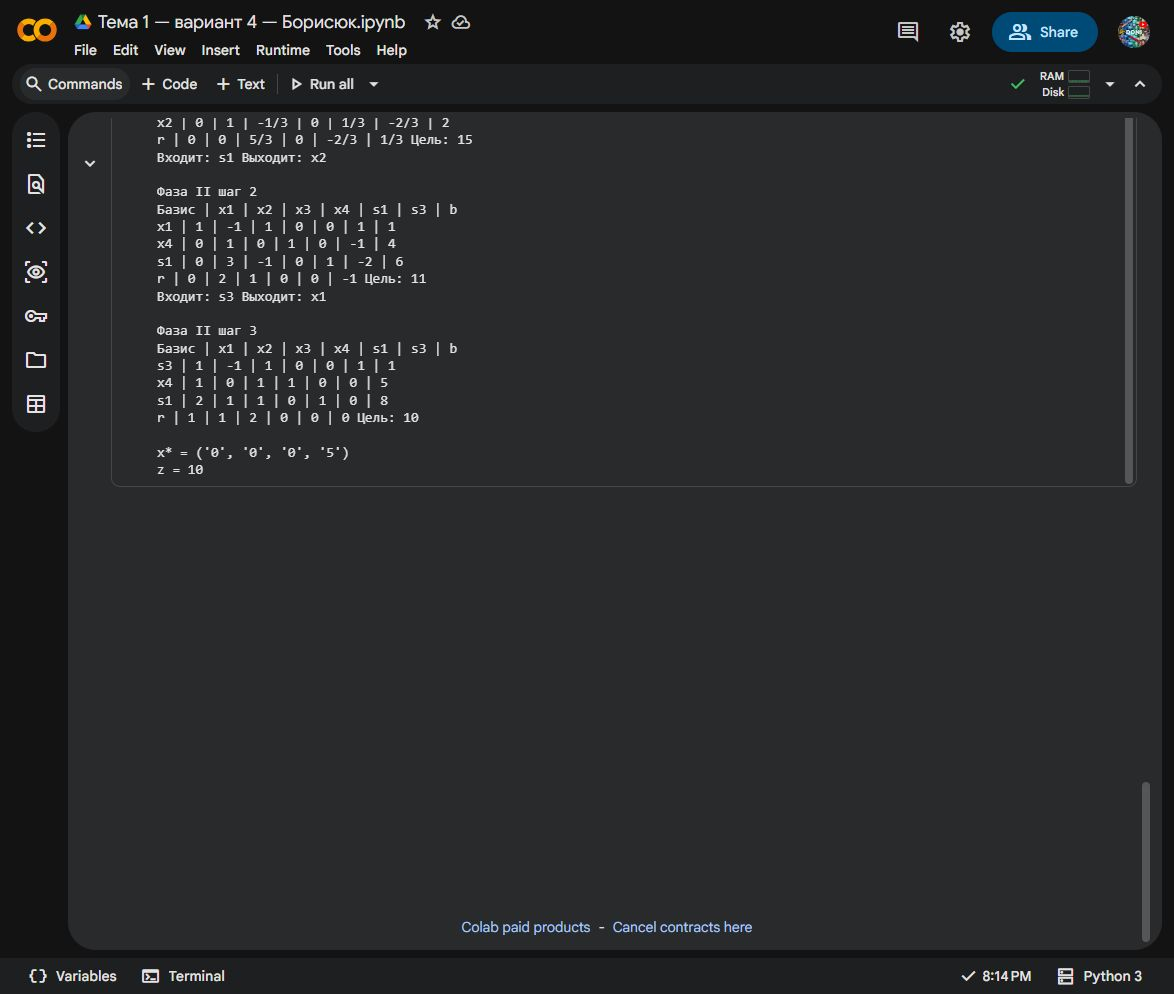
\includegraphics[width=\linewidth,trim=0 400 0 0,clip]{colab-result.png}
\end{center}
Итог: $x^*=(0,0,0,5)$, $z_{\min}=10$.
\href{https://colab.research.google.com/drive/18e0aAwlqNFxJig-vpYrivqEbL8fugkKz}{Открыть ноутбук в Google Colab}.

\par\textbf{Сравнение результатов}\par

\begin{center}
\begin{tabular}{l|c|c}\hline
Метод & Оптимальная точка & Значение цели\\\hline
Вручную & $(0,0,0,5)$ & $z_{\min}=10$\\
Excel Solver & $(0,0,0,5)$ & $z_{\min}=10$\\
Python & $(0,0,0,5)$ & $z_{\min}=10$\\
Двойственная задача & $(0,2,0)$ & $D_{\max}=10$\\\hline
\end{tabular}
\end{center}
\newpage
\par\textbf{Код программы. Часть 1}\par

\begin{Verbatim}[fontsize=\scriptsize,breaklines=true,breakanywhere=true]
# Точные дроби для вычислений
from fractions import Fraction as F

# Приводим ограничения к каноническому виду
def canonicalize(A, b, senses, c, direction='min'):
    A = [[F(v) for v in row] for row in A]
    b = list(map(F, b)); senses = list(senses)
    n = len(c); names = [f'x{i+1}' for i in range(n)]
    # Если правая часть отрицательная, меняем знак строки
    for i in range(len(b)):
        if b[i] < 0:
            A[i] = [-v for v in A[i]]; b[i] *= -1
            senses[i] = {'<=':'>=','>=':'<=','=':'='}[senses[i]]
    # Добавляем запас или избыток
    for i,s in enumerate(senses):
        if s not in ('<=','>=','='): raise ValueError('Unknown relation')
        if s != '=':
            for j,row in enumerate(A): row.append(F((1 if s=='<=' else -1) if i==j else 0))
            names.append(f's{i+1}')
    cost = [F(v)*(1 if direction=='min' else -1) for v in c] + [F(0)]*(len(names)-n)
    return A,b,cost,names

# Строим начальный базис и вспомогательную задачу
def auxiliary_problem(A,b,names):
    m=len(b); n=len(names); basis=[]; missing=[]
    # Ищем единичные столбцы; где их нет, добавляем искусственные
    for i in range(m):
        cols=[j for j,name in enumerate(names) if name.startswith('s') and
              all(A[k][j]==int(k==i) for k in range(m))]
        if cols: basis.append(cols[0])
        else: basis.append(n+len(missing)); missing.append(i)
    T=[row+[F(int(i==k)) for k in missing]+[b[i]] for i,row in enumerate(A)]
    return T,basis,[F(0)]*n+[F(1)]*len(missing),names+[f'a{k+1}' for k in missing]
\end{Verbatim}
\begin{Verbatim}[fontsize=\scriptsize,breaklines=true,breakanywhere=true]
# Считаем оценки и значение цели
def reduced_costs(T,basis,cost):
    r=[cost[j]-sum(cost[basis[i]]*T[i][j] for i in range(len(T))) for j in range(len(cost))]
    z=sum(cost[basis[i]]*T[i][-1] for i in range(len(T)))
    return r,z

# Пересчитываем таблицу по разрешающему элементу
def pivot(T,basis,row,col):
    p=T[row][col]; T[row]=[v/p for v in T[row]]
    # Обнуляем остальные элементы разрешающего столбца
    for i in range(len(T)):
        if i!=row:
            k=T[i][col]; T[i]=[v-k*w for v,w in zip(T[i],T[row])]
    basis[row]=col

def simplex(T,basis,cost,names,phase,history):
    for step in range(1000):
        r,z=reduced_costs(T,basis,cost)
        entry={'phase':phase,'step':step,'names':names[:],'basis':[names[i] for i in basis],
               'T':[[str(v) for v in row] for row in T],'r':[str(v) for v in r],'z':str(z)}
        history.append(entry)
        # 1. Выбираем первый столбец с отрицательной оценкой
        cols=[j for j,v in enumerate(r) if v<0]
        if not cols: return
        col=min(cols)  # берём первый подходящий столбец
        # 2. Ищем строку по минимальному отношению
        rows=[i for i in range(len(T)) if T[i][col]>0]
        if not rows: raise ValueError('Objective unbounded')
        row=min(rows,key=lambda i:(T[i][-1]/T[i][col],basis[i]))  # берём минимум
        entry['enter']=names[col]; entry['leave']=names[basis[row]]
        entry['ratios']=[str(T[i][-1]/T[i][col]) if T[i][col]>0 else '—' for i in range(len(T))]
        # 3. Пересчитываем таблицу и меняем базис
        pivot(T,basis,row,col)
    raise RuntimeError('Iteration limit')
\end{Verbatim}

\newpage
\par\textbf{Код программы. Часть 2}\par

\begin{Verbatim}[fontsize=\scriptsize,breaklines=true,breakanywhere=true]
# Удаляем искусственные переменные перед основной задачей
def main_problem(T,basis,n):

    for i in range(len(T)-1,-1,-1):
        if basis[i]>=n:
            if T[i][-1]!=0: raise ValueError('Infeasible')
            cols=[j for j in range(n) if j not in basis and T[i][j]!=0]
            if cols: pivot(T,basis,i,min(cols))
            else: T.pop(i); basis.pop(i)
    return [row[:n]+[row[-1]] for row in T],basis

# Выполняем обе фазы симплекс-метода
def solve_lp(A,b,senses,c,direction='min'):
    C,rhs,cost,names=canonicalize(A,b,senses,c,direction)
    T,basis,aux_cost,aux_names=auxiliary_problem(C,rhs,names)
    # 1. Решаем вспомогательную задачу
    history=[]; simplex(T,basis,aux_cost,aux_names,'I',history)
    if reduced_costs(T,basis,aux_cost)[1]!=0: raise ValueError('Infeasible')
    # 2. Возвращаемся к исходной цели
    T,basis=main_problem(T,basis,len(names))
    # 3. Решаем основную задачу
    simplex(T,basis,cost,names,'II',history)
    # Считываем оптимальную точку из базиса
    x=[F(0)]*len(names)
    for i,j in enumerate(basis): x[j]=T[i][-1]
    return x[:len(c)],sum(F(v)*u for v,u in zip(c,x)),history
\end{Verbatim}
\begin{Verbatim}[fontsize=\scriptsize,breaklines=true,breakanywhere=true]
# Данные варианта 4
A = [[2, 1, 1, 0], [1, 0, 1, 1], [0, 1, 0, 1]]
b = [8, 5, 4]
senses = ['<=', '=', '>=']
c = [3, 1, 4, 2]
x, z, history = solve_lp(A, b, senses, c)

# Выводим таблицы и ответ
for t in history:
    print('Фаза', t['phase'], 'шаг', t['step'])
    print('Базис | ' + ' | '.join(t['names']) + ' | b')
    for name, row in zip(t['basis'], t['T']):
        print(name + ' | ' + ' | '.join(row))
    print('r | ' + ' | '.join(t['r']), 'Цель:', t['z'])
    if 'enter' in t:
        print('Входит:', t['enter'], 'Выходит:', t['leave'])
    print()
print('x* =', tuple(map(str, x)))
print('z =', z)
\end{Verbatim}
\par\textbf{Рефлективный вывод}\par

Я разобрал построение начального базиса для равенства и ограничения
со знаком $\ge$. Наиболее трудным был пересчёт строк и оценок.
Для проверки сравнил ручные таблицы с Python, а итоговый ответ --- с Excel Solver.
При построении двойственной задачи проследил, как знаки исходных ограничений
определяют знаки двойственных переменных. Совпадение целей и условия
дополняющей нежёсткости подтвердили оптимальность найденных точек.



\end{document}
